\section{Approach}


\subsection{Packages}
We have extensively used python machine learning and data-science libraries throughout this project.

\begin{itemize}
    \item \textit{numpy} and \textit{pandas} are used to handle dataset and perform operations
    \item \textit{seaborn} and \textit{matplotlib} are used to visualize the dataset and output results
    \item \textit{sklearn} and \textit{xgboost} are used to run machine learning algorithms
\end{itemize}

\subsection{Data Cleaning and Pre-processing}

We have used data clipping to remove skewness in features. Columns \textit{AoCa Agatston} and \textit{Liver HU (Median)} are clipped at 99th percentile.

Moreover, the sparse nature of the dataset prompted us to fill \textit{NULL} values in CT data using the corresponding mean.

We have also used the iterative imputing strategy \cite{imputing} to fill null values in a few CT features. This type of imputing is useful when we know that a feature is dependent on other features. In this dataset, we have filled the NULL values in CT features using dependent clinical features. First, we get the correlation heatmap of all the features. Using this, we determine the features on which a CT feature is dependent. We will use these dependent features as related columns and apply \textit{sklearn.IterativeImpute}r. Under the hood, iterative imputer fits a linear regression model on non NULL values of related clinical features as 'features' and the CT feature as the 'target'. This ensures a more realistic NULL values as opposed to filling everything just by mean.
For example, we fill the NULL values in 'VAT/SAT ratio' using 'Muscle\_Area' and 'Sex' features.
We have also used correlation heatmap \ref{fig:heatmap} to drop features that are highly correlated and to add new features. We have removed TAT area and Total\_body\_area and added a new feature 'TAT area/Total\_body\_area'

\begin{figure}[h]
\centering
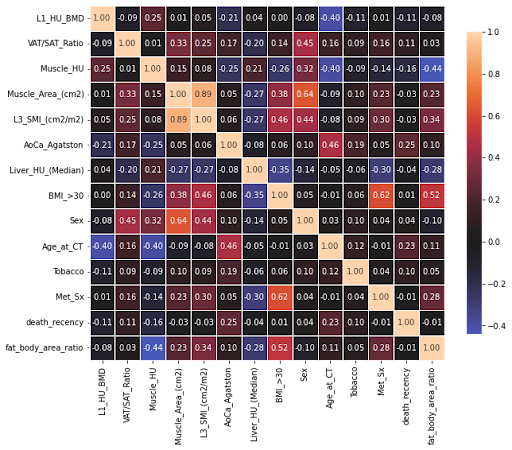
\includegraphics[width=0.8\textwidth]{images/heatmap.png}
\caption{Feature Heatmap}
\label{fig:heatmap}
\end{figure}

\subsection{Methodology - Predicting Death, Diabetes and Heart Attack}

For each 3 predictions, we first use only CT data, and then take the results again with CT + Clinical data. Our experiment involves running 3 algorithms, and comparing their corresponding RMSE(Root Mean Square Error)
\begin{enumerate}
    \item Linear Regression
    \item Support Vector Regressor
    \item XGBoost
\end{enumerate}

For each 3 predictions, we split the original dataset of size 9223 items in 80-20 train/test fashion. It includes both \textit{NULL} and \textit{NON-NULL} key columns. For example, for column \textit{DEATH [d from CT]} we have
\begin{itemize}
    \item Train Data - 7363, 6944 NULL, 419 NON-NULL
    \item Test Data - 1860, 1730 NULL, 130 NON-NULL
\end{itemize}

\subsubsection{Approach-1:}
We don't perform any other modification or data pre-processing in this approach.

For each 3 predictions, we perform the following operations:
\begin{enumerate}
    \item We train our model \textbf{only on NON-NULL training data} and test on NULL test data.
    \item We compare the distribution of values computed in the previous step with that of the NON-NULL test data
\end{enumerate}

\subsubsection{Approach-2: Recency}
In this approach, we introduced a new column \textit{recency}.
\[ death\_recency = 1 / DEATH[d\_from\_ CT]  \]
\[ diabetes\_recency = 1 /  DX\_Date[d\_from\_ CT]  \]
\[ heart\_attack\_recency = 1 / MI\_DX\_Date[d\_from\_ CT]  \]

This gives us the chance to fill all NULL values with zeros. However, it results in skewed data - Fig \ref{fig:recency_skewness_before_after_fix}. Hence, we transformed non-zero values (using Box-cox transform) to a more uniform distribution. Later, we sub-sampled zero samples to be equal to non-zero samples. This provides us with different training/test number of samples than the original. For example, for \textit{death\_recency} we got 838 training samples and 1860 test samples.

\begin{figure}[H]
	\def\imgwidth{0.5\linewidth}
% 	\setlength\tabcolsep{2pt}
	\centering
	\begin{tabular}{cc}
		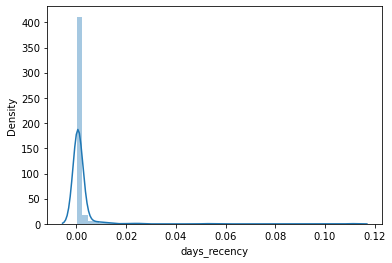
\includegraphics[width=0.4\linewidth]{images/recency_skewed.png}
		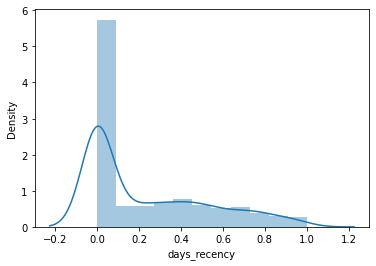
\includegraphics[width=0.4\linewidth]{images/recency_fixed.png} \\
	\end{tabular}
	\caption{left - skewness in recency, right - skewness made better}
	\label{fig:recency_skewness_before_after_fix}
\end{figure}

For each 3 predictions, we perform the following operations:
\begin{enumerate}
    \item We train our model on the \textbf{entire training data} and test on NULL test data.
    \item We compare the distribution of values computed in the previous step with that of the NON-NULL test data
\end{enumerate}

\subsection{Methodology - Deriving Biological Age}
We split the dataset into train and test using \textit{DEATH [d from CT]} column. The data item with non-empty value will go into training data, and rest will be used to check the effectiveness of the methodology. Based on this, we split the original dataset of size 9223 into 549 training items and 8674 test items.

We made few intuitive assumptions:
\begin{enumerate}
    \item People die when they hit biological age 100. Healthy people can slowdown the bio age and that is how some humans live more than 100 chronological age. This gives us \textit{max\_bio\_age\_in\_days} = 36500
    \item Higher the \textit{DEATH[d from CT]}, higher the patient has \textit{ bio\_days\_left} to live
\end{enumerate}

Based on this assumption, we define the biological age for training data as the function of \textit{bio\_days\_left}.

\[ bio\_age = max\_bio\_age\_in\_days - bio\_days\_left  \]

\[ bio\_age\_left = A + C*(1-\exp^{-k*x}) \]

Here, \textit{bio\_days\_left} follows exponential decay 
function(increasing) form as shown in Fig - \ref{fig:exp_decay}

\begin{figure}[H]
\centering
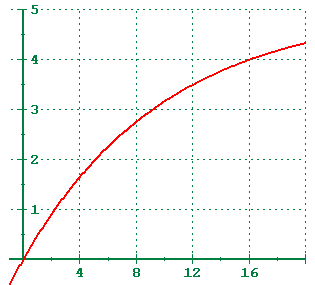
\includegraphics[width=0.3\textwidth]{images/exp_fn.png}
\caption{Example of a exponential decay increasing form plot}
\label{fig:exp_decay}
\end{figure}


We calculate \textit{bio\_days\_left} for training data, and then apply 2 the following 2 algorithms
\begin{enumerate}
    \item Linear Regression
    \item {XGBoost}
\end{enumerate}



